% IEEE conference paper. Build: pdflatex main.tex (twice). Figures: python3 report/ieee/make_ieee_figures.py
\documentclass[conference,onecolumn,11pt]{IEEEtran}
\usepackage{cite}
\usepackage{amsmath,amssymb}
\usepackage{graphicx}
\usepackage{booktabs}
\usepackage{multirow}
\usepackage{url}

\begin{document}

\title{Direction-Aware Graph Representation for Deep Reinforcement Learning-Based Droplet Routing on MEDA Biochips}

\author{\IEEEauthorblockN{Aman Bihari, Deepak, Deepak and Ankur Gupta}
\IEEEauthorblockA{Department of Computer Science and Engineering\\
Netaji Subhas University of Technology, New Delhi, India}}

\maketitle

\begin{abstract}
Micro-electrode-dot-array (MEDA) biochips move nanolitre droplets across a grid of
micro-electrode cells (MCs) whose electrodes degrade with use. Deep reinforcement learning
has been applied to route droplets on such chips by encoding the chip state as an image
with a convolutional neural network (CNN) and training the policy with proximal policy
optimization (PPO). This paper represents the chip instead as a graph with one node per MC
and eight-neighbour edges, and encodes it with a direction-aware graph convolutional network
(GCN) that applies a separate weight matrix to each neighbour direction, followed by global
max pooling. We show that isotropic message passing is insufficient, because it yields an
embedding that is invariant to the mirror and rotation symmetries of the chip, which
motivates direction-specific weights, and that the direction-aware encoder is equivalent to a fully
convolutional network with global max pooling. With the simulator, reward and PPO learner
unchanged, the direction-aware GCN, with 76\,k encoder parameters against 29.7\,M for the
CNN, converged in all five training seeds on $30\times30$ chips after
$134\pm24$\,k environment steps, whereas the CNN converged only after 819\,k steps in a
single 100-epoch run (one seed). With a budget of 40 epochs, it routed on average at least
99.6\% of held-out jobs (every run at least 99.2\%) on chips of up to $100\times100$ MCs, while the success rate of the CNN fell from 87.4\% to
15.6\%; on $120\times120$ chips it reached 94.2\% against 10.2\%. On chips with 10\% and
20\% faulty MCs it routed 94.0\% and 82.2\% of the jobs against 80.4\% and 69.3\%.
\end{abstract}

\begin{IEEEkeywords}
Digital microfluidics, MEDA biochips, droplet routing, deep reinforcement learning, graph
convolutional networks.
\end{IEEEkeywords}

\section{Introduction}
Digital microfluidic biochips automate biochemical protocols by manipulating discrete
droplets on an array of electrodes through electrowetting-on-dielectric
\cite{pollack2000,chakrabarty2006}. The micro-electrode-dot-array (MEDA) architecture
divides the array into thousands of identical micro-electrode cells (MCs), each with its own
actuation and sensing circuitry \cite{wang2011,li2017}. A droplet covers a rectangle of MCs
and is moved by actuating the MCs adjacent to its leading edge. Repeated actuation degrades
an MC, so that the force it exerts decreases and droplet movement becomes stochastic
\cite{elfar2023}. A router must therefore choose, at every control cycle, a direction that
brings the droplet to its goal quickly while accounting for the sensed health of the MCs.

Elfar et al.\ \cite{elfar2022date,elfar2023} formulated this task as a reinforcement-learning
problem: a convolutional neural network (CNN) encodes the MC health, droplet and goal as a
three-channel image, and proximal policy optimization (PPO) \cite{schulman2017} learns the
routing policy. The CNN treats the chip as an image of fixed size: chips of any size are
resampled to $30\times30$ pixels, and 29.5 of the 29.7 million parameters of the network
lie in a fully connected layer whose size is tied to that resolution.

A MEDA chip, however, is physically a set of cells with fixed neighbourhoods, which is
naturally described as a graph. This paper investigates a graph representation of the chip
state as the input of the PPO learner. Its contributions are as follows.
\begin{itemize}
\item A graph formulation of MEDA droplet routing with one node per MC and eight-neighbour
      edges, encoded by a direction-aware graph convolutional network (GCN) with global max
      pooling whose 76\,k parameters do not depend on the chip size.
\item An analysis showing that isotropic message passing cannot distinguish a routing job
      from its mirror images and rotations, and that the direction-aware encoder is
      equivalent to a fully convolutional network with global max pooling; both statements
      are verified by automated tests.
\item A controlled comparison with the CNN--PPO method of \cite{elfar2023} on chips of
      $30\times30$ to $120\times120$ MCs and on chips with faulty MCs, with up to five
      training seeds, together with a training comparison of our implementation of the
      baseline against the authors' original implementation \cite{elfarcode}.
\end{itemize}

\section{Related Work}
\textit{Droplet routing.} Early methods routed droplets on ideal electrode grids as part of
biochip synthesis \cite{su2006}. Elfar et al.\ \cite{elfar2021date,elfar2022tcad} modelled MC
degradation explicitly and synthesized adaptive routing strategies with stochastic games,
which are reliable but costly for large chips. Liang et al.\ applied deep reinforcement
learning to droplet routing on digital microfluidic biochips \cite{liang2020} and to the
parallel control of multiple droplets on MEDA biochips \cite{liang2021}. Elfar et al.\
\cite{elfar2022date,elfar2023} route droplets on MEDA biochips with a CNN--PPO agent that
observes the sensed MC health, uses an action space whose step size adapts to the droplet
size, and transfers learning across chip sizes.

\textit{Graph neural networks and reinforcement learning.} Message-passing networks
\cite{gilmer2017} update node embeddings from their neighbours; the GCN of Kipf and Welling
\cite{kipf2017} uses a normalized neighbourhood average, and relational GCNs
\cite{schlichtkrull2018} learn a separate weight matrix per edge type. Xu et al.\
\cite{xu2019} analysed how aggregation and readout functions limit the discriminative power
of message-passing networks, and Beaini et al.\ \cite{beaini2021} argued that isotropic
aggregation cannot capture directions. In reinforcement learning, relational inductive
biases have been introduced into deep agents \cite{zambaldi2019}, grid observations have
been represented as graphs whose edge types encode spatial relations \cite{jiang2021}, and
an edge-based graph network encodes the netlist for chip macro placement with PPO
\cite{mirhoseini2021}. To our knowledge, no prior work represents the MEDA electrode array as
a graph for a reinforcement-learning router.

\section{Problem Formulation}
\textit{Chip model.} A $W\times H$ chip holds MCs indexed by $(x,y)$. A routing job moves a
droplet, a rectangle of MCs, from a start to a goal location within a routing zone, defined
as the bounding box of start and goal enlarged by three MCs. Following \cite{elfar2023}, the
degradation of MC $(i,j)$ after $n_{ij}$ actuations and its sensed health are
\begin{equation}
  D_{ij}=\tau_{ij}^{\,n_{ij}/c_{ij}},\qquad
  H_{ij}=\min\!\big(\lfloor 2^{b} D_{ij}\rfloor,\ 2^{b}-1\big),
\end{equation}
with $\tau_{ij}\in[0.5,0.7]$, $c_{ij}\in[500,800]$ and a $b=2$-bit health sensor. A move
succeeds with a probability determined by the degradation of the MCs at the leading edge.

\textit{Markov decision process.} The state is a three-channel $W\times H$ grid holding the
MC health inside the routing zone ($H/2^{b}$, and 0 outside), the droplet and the goal. The
action is one of eight directions; the step size adapts to the droplet size and never
overshoots the goal (Algorithm~1 of \cite{elfar2023}). The reward, with the coefficients of
the reference implementation \cite{elfarcode}, is $+0.5\,\Delta d$ for a move that reduces
the distance $d$ to the goal, $0.8\,\Delta d-1$ otherwise, $-1$ for an action that would
leave the routing zone, and $+100$ on arrival. An episode ends at the goal or after
$k_{\max}=W_h+H_h$ control cycles, where $W_h\times H_h$ is the size of the routing zone.

\textit{Baseline.} The CNN of \cite{elfar2023} (Table~I there) has three $3\times3$
convolutional layers with 64, 128 and 128 filters (stride 1, zero padding, as in
\cite{elfarcode}) and a 256-unit fully connected layer; linear actor and critic heads share
it. Every chip is resampled to a $30\times30$ observation by area averaging.

\section{Direction-Aware Graph Representation}
\textit{Graph.} Each MC is a node with index $y\,W+x$ and features
$X_i=[\text{health}_i,\text{droplet}_i,\text{goal}_i]$, copied from the observation without
renormalization. Edges connect every MC to its eight spatial neighbours in both directions,
\begin{equation}
|E| = 2\big[(W-1)H + W(H-1) + 2(W-1)(H-1)\big],
\end{equation}
i.e.\ 6\,844 directed edges on a $30\times30$ chip. The graph always has the native
resolution of the chip.

\textit{Direction-aware message passing.} Each of $L=3$ layers of the direction-aware GCN
(DA-GCN) updates node $i$ as
\begin{equation}
  h_i^{(l+1)} = \mathrm{ReLU}\Big(W_0^{(l)} h_i^{(l)} + \sum_{r=1}^{8}\sum_{j\in\mathcal{N}_r(i)} W_r^{(l)} h_j^{(l)} + b^{(l)}\Big),
\end{equation}
where $\mathcal{N}_r(i)$ contains the neighbour of MC $i$ in direction $r$, if it exists,
and $h_i^{(0)}=X_i$. Directions are derived from the node indices, so the graph carries no
edge attributes. With hidden dimension $d=64$, the encoder has 75\,648 parameters for any
chip size. A global max pooling readout, $g_k=\max_i h_{i,k}^{(L)}$, gives a fixed-size
embedding $g\in\mathbb{R}^{64}$, from which linear heads compute the action probabilities
and the state value as in the baseline. The simulator, reward, action space and PPO settings
are those of the baseline, so the encoder is the only difference between the two methods.

\textit{Why isotropic message passing is insufficient.} Every mirror and rotation of a square
chip (the dihedral group $D_4$) maps the eight-neighbour grid onto itself. An isotropic GCN
\cite{kipf2017}, which weights all neighbours alike, therefore produces node embeddings of a
transformed job that are a permutation of those of the original job, and any readout that
ignores node order assigns both the same graph embedding. A policy computed from this
embedding cannot distinguish a job from its mirror images and rotations: for a goal that
lies straight along one axis from the droplet, the eight transformed jobs require each of the
four axis directions twice, so such a policy selects the direction of the goal with
probability at most $1/4$ on average over them.

\textit{Equivalence with convolution.} Each direction-aware layer is a $3\times3$
convolution with stride 1 and zero padding: $W_0^{(l)}$ is the centre tap, $W_r^{(l)}$ is
the tap at the position of the neighbour in direction $r$, and a neighbour that does not
exist at the chip border contributes nothing, as zero padding does. The encoder is
therefore a three-layer fully convolutional network followed by global max pooling, whose
convolutional layers are translation-equivariant and whose size is independent of the chip
size; a similar correspondence was
noted by Jiang et al.\ \cite{jiang2021}. Both this equivalence and the invariance of the
isotropic GCN are verified numerically by automated tests. Each node embedding depends on
the $7\times7$ block of MCs within three hops.

\section{Experimental Setup}
The simulator is implemented as a Gymnasium environment \cite{towers2024}, and both methods
are trained with the PPO implementation of Stable-Baselines3 \cite{raffin2021};
Table~\ref{tab:setup} lists the settings. Training proceeds in epochs of $2^{14}$
environment steps. After every epoch the deterministic policy is evaluated on a fixed set of
500 jobs; this evaluation determines the learning-rate decay and the convergence point,
defined as the first of three consecutive evaluations with at least 95\% success. After
training, each final model is evaluated on 500 held-out jobs drawn with a separate random
seed, identical for both methods; these held-out results are reported unless stated
otherwise. Results over several seeds are given as mean $\pm$ sample standard deviation, and
differences are tested with Welch's $t$-test across seeds or, for single runs, with an
exact McNemar test on the paired jobs. The CNN runs at $100\times100$ and $120\times120$
and the runs with seed 0 at $30\times30$ to $60\times60$ (40 epochs) were trained on Tesla
T4 GPUs; all other runs used an A100 server. The DA-GCN runs at $100\times100$ and
$120\times120$ were repeated there for the full 40 epochs because the T4 runs had reached a
session time limit after 34 and 21 epochs.

\begin{table}[!htbp]
\caption{Experimental Settings}
\label{tab:setup}
\centering\footnotesize
\begin{tabular}{@{}p{2.6cm}p{11cm}@{}}
\toprule
Item & Value \\ \midrule
Chips & $30\times30$ to $120\times120$ MCs; healthy, or 10\%/20\% fully degraded MCs in $2\times2$ clusters redrawn every episode \\
Droplets & 9 sizes, $w,h\in\{2,\dots,6\}$, $w/h\in[0.8,1.25]$ \\
Observation & CNN: $30\times30$ (resampled); GCN: native grid \\
PPO & 8 environments, 64 steps, minibatch 32, 4 epochs, $\gamma=0.99$, $\lambda=0.95$, entropy 0.01, clip 0.2, value coefficient 0.25 \\
Learning rate & $3.5\times10^{-4}$, $\times0.7$ after an epoch with $>99\%$ success, floor $10^{-6}$ \\
Budget & 40 epochs ($655\,360$ steps); 25 epochs in the five-seed $30\times30$ study; 20 fine-tuning epochs on faulty chips \\
Seeds & 5 at $30\times30$ (25 epochs), $50\times50$, $60\times60$ and on faulty chips; 1 otherwise \\
Hardware & NVIDIA Tesla T4 and A100 GPUs, AMD EPYC 7742 CPUs \\
\bottomrule
\end{tabular}
\end{table}

\section{Results}
We first validate our implementation of the baseline and then compare the two methods on $30\times30$ chips, across chip sizes and on chips with faulty MCs.

\subsection{Validation of the Baseline Implementation}
To verify our implementation of the baseline, it and the authors' original implementation
\cite{elfarcode} (commit \texttt{1667016}, unmodified) were trained with the settings of the
authors' logged $30\times30$ run for 40 epochs, with three seeds each. The original
implementation at this commit uses a smaller CNN (32, 64 and 64 filters, FC 128) and a
learning-rate factor of 0.7; our first set of runs used the Table~I network and the factor
0.5 of the authors' log, and a second set used the original network and factor.
Table~\ref{tab:reference} and Fig.~\ref{fig:reference} show the results. Our implementation
reached 95\% success earlier on average (Welch's $t$-test, $p=0.089$ and $0.039$) and ended
0.8 and 1.2 percentage points lower; after Holm correction over the four metrics, only the
lower final success of the second set remains significant ($p=0.028$). The comparison gives
no indication that our implementation of the baseline learns more slowly than the original.

\begin{table}[!htbp]
\caption{Comparison With the Authors' Original Implementation (Three Seeds Each)}
\label{tab:reference}
\centering\footnotesize
\setlength{\tabcolsep}{3pt}
\begin{tabular}{@{}lcccc@{}}
\toprule
Implementation & First epoch & Converged & Final & Final \\
 & $\geq$95\% & (epoch) & success (\%) & cycles \\ \midrule
Original \cite{elfarcode} & $25.7\pm3.1$ & $25.7\pm3.1$ & $99.81\pm0.15$ & $7.95\pm0.61$ \\
Ours, Table~I CNN & $20.3\pm0.6$ & $23.3\pm1.5$ & $99.05\pm0.26$ & $8.42\pm0.14$ \\
Ours, original CNN & $18.7\pm1.5$ & $20.7\pm3.5$ & $98.64\pm0.28$ & $8.70\pm0.20$ \\
\bottomrule
\end{tabular}
\end{table}

\begin{figure}[!htbp]
\centering
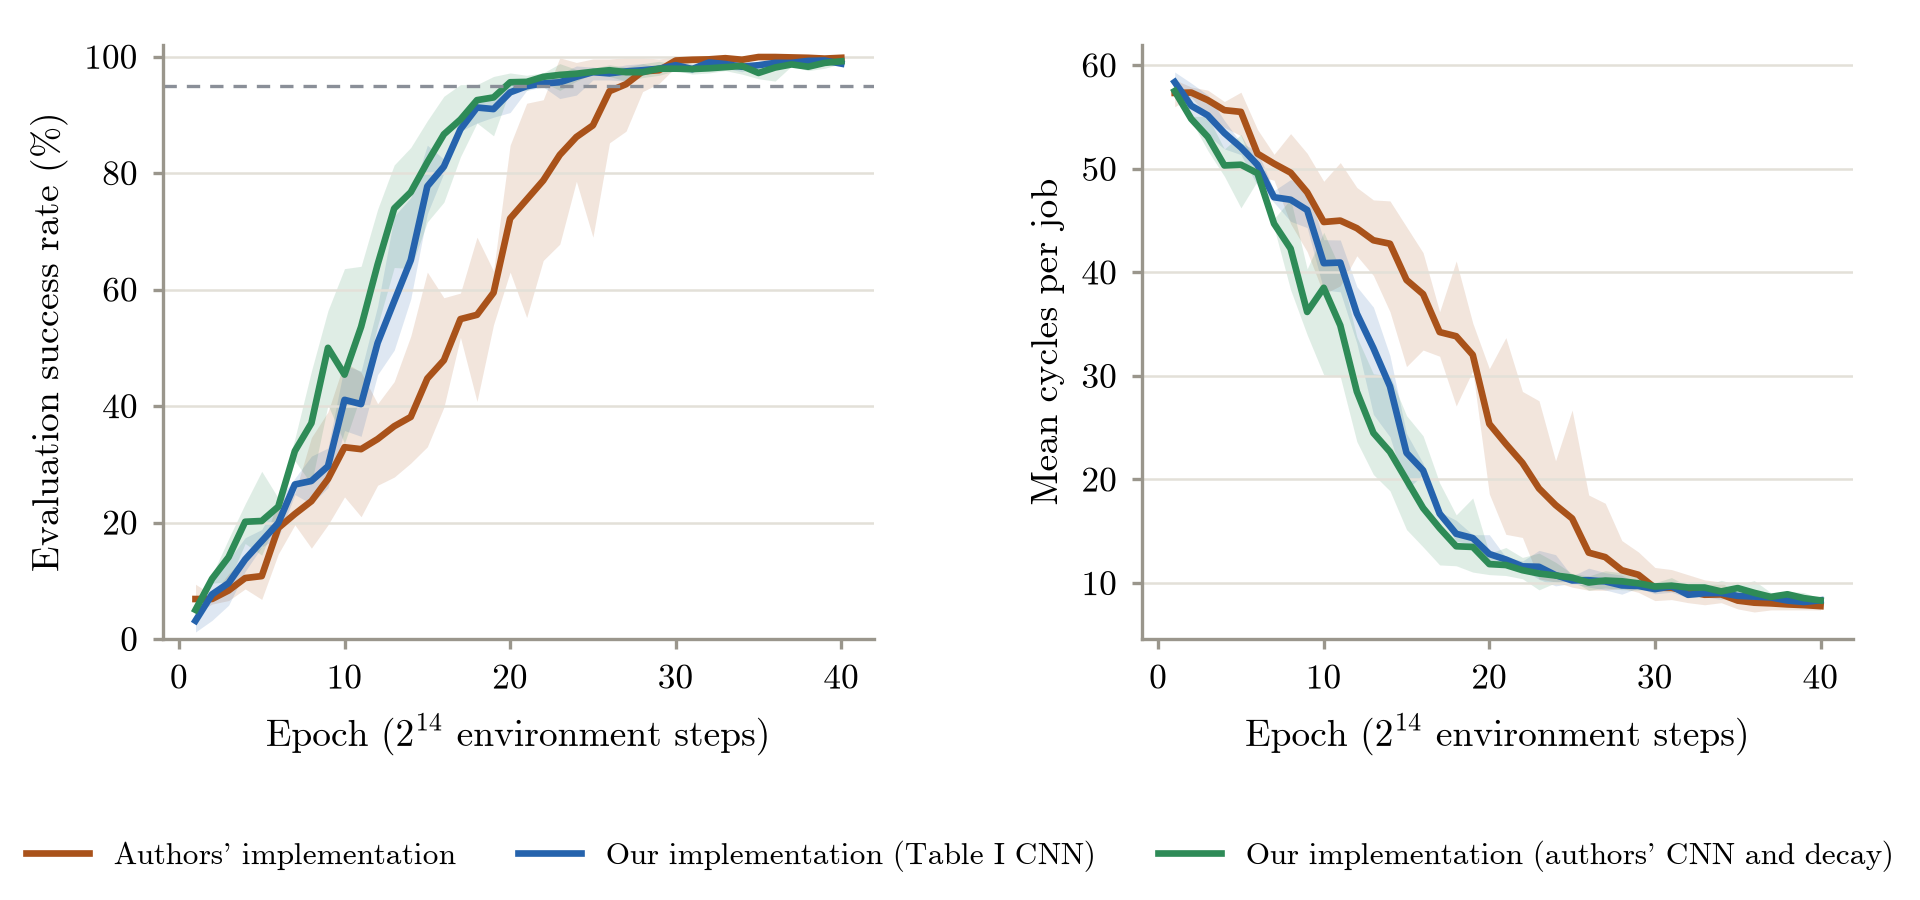
\includegraphics[width=0.9\textwidth]{figures/reference_test.png}
\caption{Per-epoch success rate (left) and mean cycles (right) of the authors' original
implementation and of our implementation of the baseline under the settings of the
authors' logged run (three seeds each; line: mean, band: minimum to maximum). The dashed
line marks 95\% success.}
\label{fig:reference}
\end{figure}


\begin{figure}[!htbp]
\centering
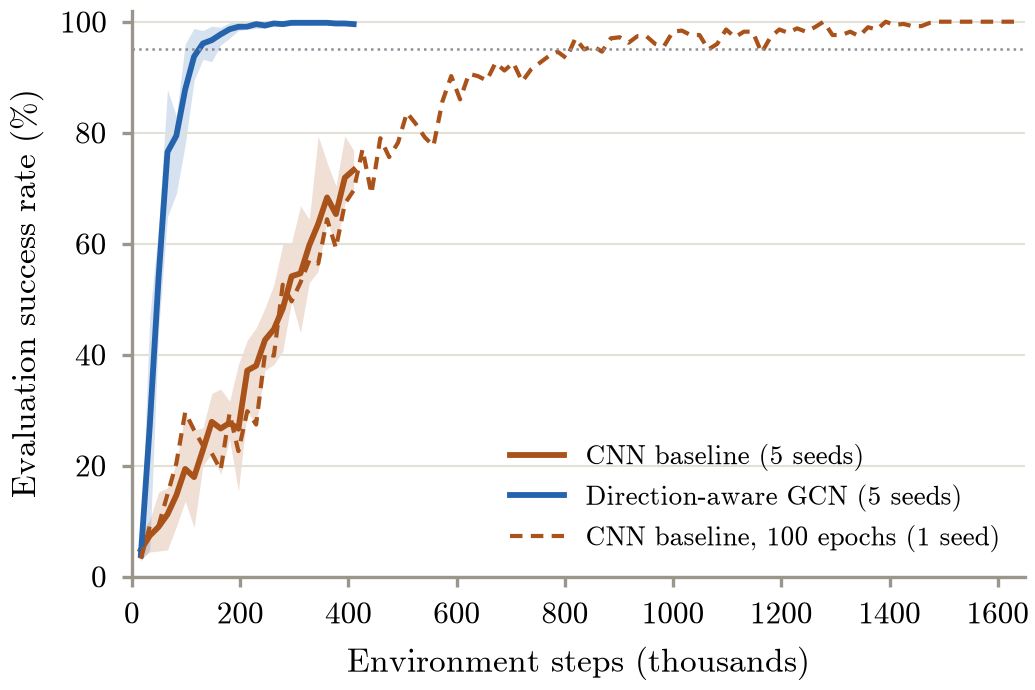
\includegraphics[width=0.62\textwidth]{figures/curves_30x30.png}
\caption{Per-epoch evaluation success rate on $30\times30$ chips: five seeds of each method
(line: mean, band: minimum to maximum) and a 100-epoch run of the CNN. The dotted line marks
the 95\% convergence threshold.}
\label{fig:curves}
\end{figure}

\begin{figure}[!htbp]
\centering
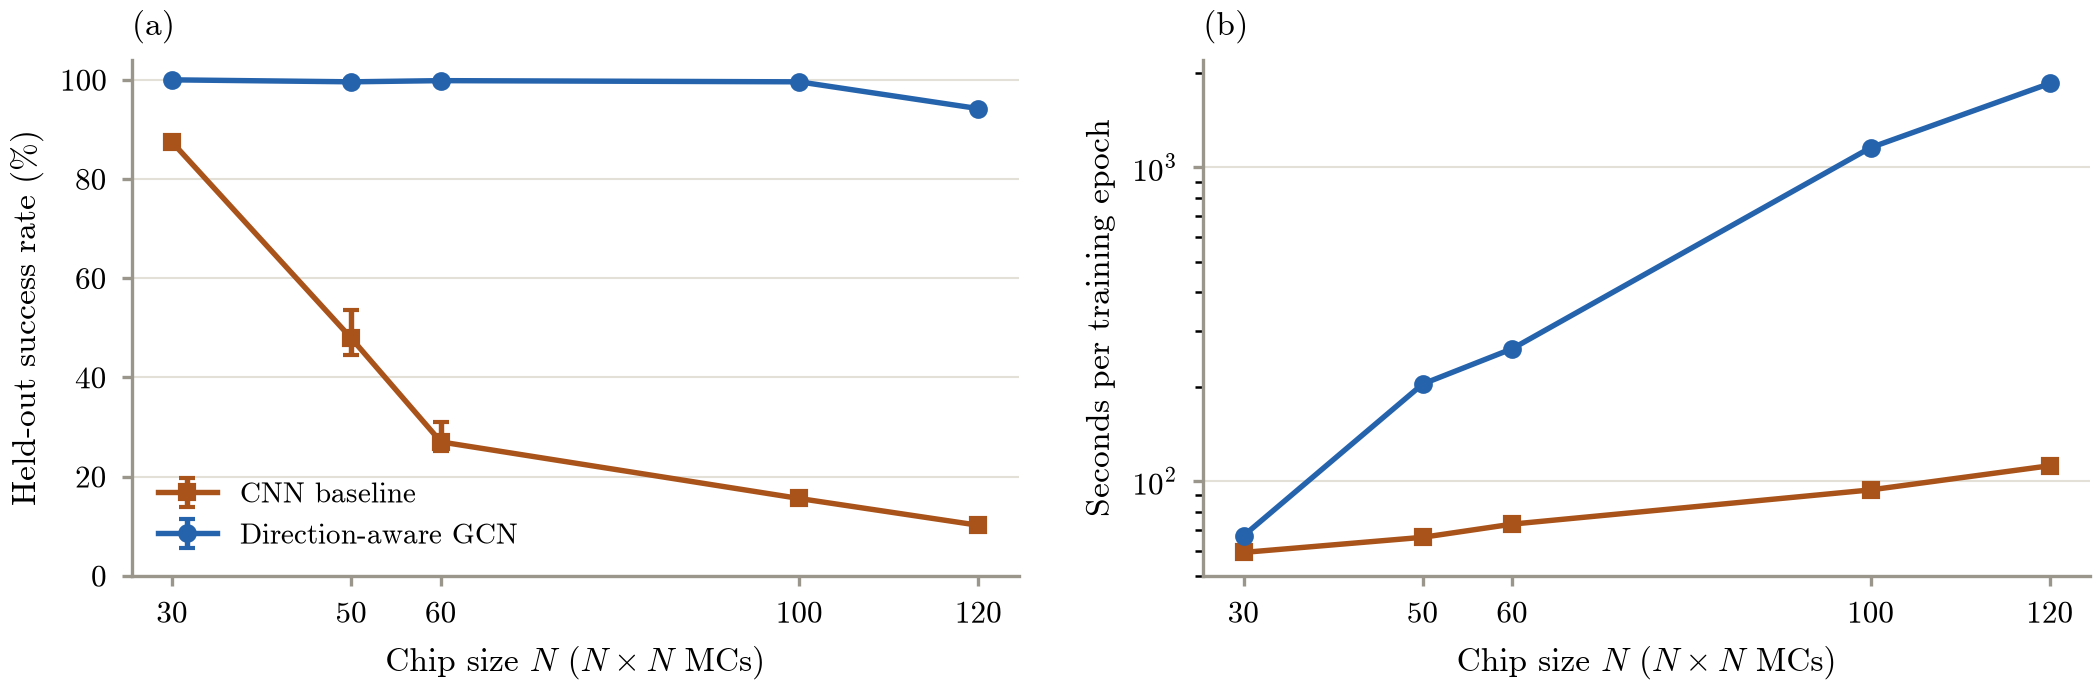
\includegraphics[width=0.9\textwidth]{figures/chip_size.png}
\caption{Chip-size study (40 epochs): (a) held-out success rate (mean and range over five
seeds at $50\times50$ and $60\times60$, one seed otherwise); (b) mean wall-clock time per
epoch (training and 500-job evaluation) on a Tesla T4 GPU, logarithmic scale.}
\label{fig:sizes}
\end{figure}

\subsection{Learning Speed on $30\times30$ Chips}
Table~\ref{tab:seeds30} and Fig.~\ref{fig:curves} compare the two methods over five seeds
with a budget of 25 epochs. The direction-aware GCN met the convergence criterion in every
seed, between epochs 6 and 10, and routed $99.9\pm0.1\%$ of the held-out jobs. The CNN
converged in no seed and routed $73.7\pm4.0\%$ ($p=1.2\times10^{-4}$); its highest and the
GCN's lowest success rates are 21 percentage points apart. When the CNN was trained for
100 epochs with one seed, it met the convergence criterion at epoch 50, after 819\,k
environment steps, about six times as many as the GCN, and finally routed 100\% of the
held-out jobs in 9.72 cycles. On $30\times30$ chips the advantage of the graph encoder is
therefore its learning speed and its size, not its final performance.

\begin{table}[!htbp]
\caption{Five Seeds on Healthy $30\times30$ Chips (25 Epochs)}
\label{tab:seeds30}
\centering\footnotesize
\setlength{\tabcolsep}{3pt}
\begin{tabular}{@{}lcccc@{}}
\toprule
Method & Success & Mean & Invalid actions & Steps to \\
 & (\%) & cycles & per decision & convergence \\ \midrule
CNN & $73.7\pm4.0$ & $18.62\pm0.92$ & $0.18\pm0.03$ & none of 5 \\
DA-GCN & $\mathbf{99.9\pm0.1}$ & $\mathbf{10.16\pm0.41}$ & $\mathbf{0.003\pm0.003}$ & $\mathbf{134\pm24}$\,k \\
\bottomrule
\end{tabular}
\end{table}



\subsection{Chip Size}
Both methods were trained from scratch with 40 epochs on chips of $30\times30$ to
$120\times120$ MCs (Table~\ref{tab:sizes}, Fig.~\ref{fig:sizes}). The success rate of the
CNN, which observes every chip resampled to $30\times30$, fell from 87.4\% to 10.2\%, and it
converged at no size. The direction-aware GCN routed on average at least 99.6\% of the
held-out jobs (every run at least 99.2\%) up to $100\times100$ MCs and converged at each of these sizes; on $120\times120$ chips it
reached 94.2\% without meeting the convergence criterion, with per-epoch success between
89.8\% and 95.6\% over the last five epochs. Over five seeds the CNN routed
$47.9\pm3.7\%$ against $99.6\pm0.3\%$ for the GCN on $50\times50$ chips and $27.0\pm2.5\%$ against $99.8\pm0.2\%$ on
$60\times60$ chips ($p=5.2\times10^{-6}$ and $2.7\times10^{-7}$). For the single-seed sizes,
the jobs solved by only one method were almost all solved by the GCN (exact McNemar test,
$p<10^{-18}$ at every size).

\begin{table}[!htbp]
\caption{Chip-Size Study (40 Epochs; Held-Out Success in \%, Mean Cycles in Parentheses)}
\label{tab:sizes}
\centering\footnotesize
\setlength{\tabcolsep}{3pt}
\begin{tabular}{@{}lccc@{}}
\toprule
Chip & Seeds & CNN & DA-GCN \\ \midrule
$30\times30$ & 1 & 87.4 (14.52) & \textbf{100.0 (9.84)} \\
$50\times50$ & 5 & $47.9\pm3.7$ ($38.94$) & $\mathbf{99.6\pm0.3}$ (\textbf{17.25}) \\
$60\times60$ & 5 & $27.0\pm2.5$ ($53.76$) & $\mathbf{99.8\pm0.2}$ (\textbf{21.03}) \\
$100\times100$ & 1 & 15.6 (86.47) & \textbf{99.6 (35.05)} \\
$120\times120$ & 1 & 10.2 (108.61) & \textbf{94.2 (47.24)} \\ \midrule
\multicolumn{4}{@{}p{0.6\textwidth}@{}}{DA-GCN steps to convergence: 147\,k, $246\pm60$\,k, $259\pm55$\,k, 246\,k and not reached; the CNN converged at no size.}\\
\bottomrule
\end{tabular}
\end{table}


\textit{Computational cost.} The cost of the GCN grows with the number of MCs, whereas the
CNN always processes a $30\times30$ input. On a Tesla T4 an epoch (training and the 500-job evaluation) took 67\,s on
$30\times30$ chips and 1\,852\,s on $120\times120$ chips for the GCN, against 59\,s and
112\,s for the CNN (Fig.~\ref{fig:sizes}b); per forward pass, the GCN needs more
multiply--accumulate operations than the CNN (230\,M) from about $55\times55$ MCs.

\subsection{Chips With Faulty MCs}
Following the protocol of \cite[Fig.~8]{elfar2023}, the healthy $30\times30$ agent of each
seed was fine-tuned for 20 epochs on chips with 10\% or 20\% fully degraded MCs, which appear
in the health channel and must be avoided. Table~\ref{tab:faults} reports the held-out
results for five seeds. The direction-aware GCN routed 94.0\% and 82.2\% of the jobs against
80.4\% and 69.3\% for the CNN ($p=3.6\times10^{-4}$ and $3.8\times10^{-6}$), in fewer cycles.
Neither method met the convergence criterion within the 20 epochs, and the CNN started from
healthy agents that had not converged, so part of this gap is inherited from the healthy
training.

\begin{table}[!htbp]
\caption{Chips With Faulty MCs ($30\times30$, Five Seeds, 20 Fine-Tuning Epochs)}
\label{tab:faults}
\centering\footnotesize
\setlength{\tabcolsep}{3pt}
\begin{tabular}{@{}llccc@{}}
\toprule
Faulty & Method & Success & Mean & Invalid actions \\
MCs & & (\%) & cycles & per decision \\ \midrule
10\% & CNN & $80.4\pm2.9$ & $17.47\pm0.51$ & $0.102\pm0.040$ \\
 & DA-GCN & $\mathbf{94.0\pm0.5}$ & $\mathbf{13.15\pm0.18}$ & $\mathbf{0.020\pm0.013}$ \\ \midrule
20\% & CNN & $69.3\pm1.9$ & $21.81\pm0.33$ & $0.087\pm0.020$ \\
 & DA-GCN & $\mathbf{82.2\pm1.6}$ & $\mathbf{17.85\pm0.57}$ & $\mathbf{0.045\pm0.023}$ \\
\bottomrule
\end{tabular}
\end{table}

\section{Discussion and Limitations}
The results suggest that the inductive bias of the encoder, rather than its capacity,
governs how quickly the router learns: the direction-aware GCN applies the same local
rule at every position, whereas the fully connected layer of the CNN must learn the mapping
for every position separately. Several limitations qualify these findings. The comparisons
at $30\times30$ (40 epochs), $100\times100$ and $120\times120$ use one seed, and runs of the
GCN with the same seed on different platforms varied considerably on $120\times120$ chips
(per-epoch success after 21 epochs: 86.4\% on the T4, 60.6\% on the A100).
Above $30\times30$ MCs the CNN observes a resampled chip while the GCN observes the native
grid, and the two encoders also differ in readout and width, so the comparison does not
isolate the graph representation from these factors. Each chip size was trained from
scratch, unlike the transfer learning of \cite{elfar2023}. On healthy chips the sensed
health of almost every MC stays at its maximum during an episode, and the faulty chips
contain only fully degraded MCs; the gradual wear of MCs over many bioassays is not yet
exercised. Finally, within the 20-, 25- and 40-epoch budgets the learning-rate decay was
triggered only for the GCN, the only method that exceeded 99\% success; in the 100-epoch run
of the CNN it was first triggered at epoch 79.

\section{Conclusion}
This paper proposed a direction-aware graph representation of the MEDA electrode array for
reinforcement-learning-based droplet routing. Direction information is necessary in
message passing, since isotropic aggregation cannot distinguish a routing job from its mirror
images, and the resulting encoder is a size-independent fully convolutional network with
76\,k parameters. Compared with the CNN--PPO method of \cite{elfar2023} with the same
simulator, reward and PPO settings, it converged in about one sixth of the environment steps
on $30\times30$ chips (five GCN seeds against a single 100-epoch CNN run), maintained on
average at least 99.6\% success up to $100\times100$ MCs within a budget at which the CNN fell to
15.6\%, and routed more jobs on chips with faulty MCs. Future work will extend the multi-seed
evaluation to the largest chips, separate the effects of representation, readout and
observation resolution, evaluate transfer across chip sizes without retraining, and study
routing under gradual degradation and on bioassay benchmarks.

\begin{thebibliography}{99}
\bibitem{pollack2000} M.~G.~Pollack, R.~B.~Fair, and A.~D.~Shenderov, ``Electrowetting-based actuation of liquid droplets for microfluidic applications,'' \emph{Appl. Phys. Lett.}, vol.~77, no.~11, pp.~1725--1726, 2000.
\bibitem{chakrabarty2006} K.~Chakrabarty and F.~Su, \emph{Digital Microfluidic Biochips: Synthesis, Testing, and Reconfiguration Techniques}. Boca Raton, FL, USA: CRC Press, 2006.
\bibitem{wang2011} G.~Wang, D.~Teng, and S.-K.~Fan, ``Digital microfluidic operations on micro-electrode dot array architecture,'' \emph{IET Nanobiotechnol.}, vol.~5, no.~4, pp.~152--160, 2011.
\bibitem{li2017} Z.~Li, K.~Y.-T.~Lai, P.-H.~Yu, K.~Chakrabarty, T.-Y.~Ho, and C.-Y.~Lee, ``Droplet size-aware high-level synthesis for micro-electrode-dot-array digital microfluidic biochips,'' \emph{IEEE Trans. Biomed. Circuits Syst.}, vol.~11, no.~3, pp.~612--626, 2017.
\bibitem{elfar2023} M.~Elfar, Y.-C.~Chang, H.~H.-Y.~Ku, T.-C.~Liang, K.~Chakrabarty, and M.~Pajic, ``Deep reinforcement learning-based approach for efficient and reliable droplet routing on MEDA biochips,'' \emph{IEEE Trans. Comput.-Aided Design Integr. Circuits Syst.}, vol.~42, no.~4, pp.~1212--1222, 2023.
\bibitem{elfar2022date} M.~Elfar, T.-C.~Liang, K.~Chakrabarty, and M.~Pajic, ``Adaptive droplet routing for MEDA biochips via deep reinforcement learning,'' in \emph{Proc. Design, Autom. Test Eur. Conf. (DATE)}, 2022, pp.~640--645.
\bibitem{schulman2017} J.~Schulman, F.~Wolski, P.~Dhariwal, A.~Radford, and O.~Klimov, ``Proximal policy optimization algorithms,'' arXiv:1707.06347, 2017.
\bibitem{elfarcode} M.~Elfar, ``MEDA,'' GitHub repository, commit 1667016. [Online]. Available: \url{https://github.com/melfar87/MEDA} (accessed Oct. 2026).
\bibitem{su2006} F.~Su, W.~Hwang, and K.~Chakrabarty, ``Droplet routing in the synthesis of digital microfluidic biochips,'' in \emph{Proc. DATE}, 2006, pp.~323--328.
\bibitem{elfar2021date} M.~Elfar, T.-C.~Liang, K.~Chakrabarty, and M.~Pajic, ``Formal synthesis of adaptive droplet routing for MEDA biochips,'' in \emph{Proc. DATE}, 2021, pp.~324--329.
\bibitem{elfar2022tcad} M.~Elfar, T.-C.~Liang, K.~Chakrabarty, and M.~Pajic, ``Formal synthesis of adaptive droplet routing for MEDA biochips,'' \emph{IEEE Trans. Comput.-Aided Design Integr. Circuits Syst.}, vol.~41, no.~8, pp.~2504--2517, 2022.
\bibitem{liang2020} T.-C.~Liang, Z.~Zhong, Y.~Bigdeli, T.-Y.~Ho, K.~Chakrabarty, and R.~Fair, ``Adaptive droplet routing in digital microfluidic biochips using deep reinforcement learning,'' in \emph{Proc. Int. Conf. Mach. Learn. (ICML)}, 2020, pp.~6050--6060.
\bibitem{liang2021} T.-C.~Liang, J.~Zhou, Y.-S.~Chan, T.-Y.~Ho, K.~Chakrabarty, and C.-Y.~Lee, ``Parallel droplet control in MEDA biochips using multi-agent reinforcement learning,'' in \emph{Proc. ICML}, 2021, pp.~6588--6599.
\bibitem{gilmer2017} J.~Gilmer, S.~S.~Schoenholz, P.~F.~Riley, O.~Vinyals, and G.~E.~Dahl, ``Neural message passing for quantum chemistry,'' in \emph{Proc. ICML}, 2017, pp.~1263--1272.
\bibitem{kipf2017} T.~N.~Kipf and M.~Welling, ``Semi-supervised classification with graph convolutional networks,'' in \emph{Proc. Int. Conf. Learn. Represent. (ICLR)}, 2017.
\bibitem{schlichtkrull2018} M.~Schlichtkrull, T.~N.~Kipf, P.~Bloem, R.~van den Berg, I.~Titov, and M.~Welling, ``Modeling relational data with graph convolutional networks,'' in \emph{Proc. Eur. Semantic Web Conf. (ESWC)}, 2018, pp.~593--607.
\bibitem{xu2019} K.~Xu, W.~Hu, J.~Leskovec, and S.~Jegelka, ``How powerful are graph neural networks?'' in \emph{Proc. ICLR}, 2019.
\bibitem{beaini2021} D.~Beaini, S.~Passaro, V.~L{\'e}tourneau, W.~L.~Hamilton, G.~Corso, and P.~Li{\`o}, ``Directional graph networks,'' in \emph{Proc. ICML}, 2021, pp.~748--758.
\bibitem{zambaldi2019} V.~Zambaldi \emph{et al.}, ``Deep reinforcement learning with relational inductive biases,'' in \emph{Proc. ICLR}, 2019.
\bibitem{jiang2021} Z.~Jiang, P.~Minervini, M.~Jiang, and T.~Rockt{\"a}schel, ``Grid-to-Graph: Flexible spatial relational inductive biases for reinforcement learning,'' in \emph{Proc. Int. Conf. Auton. Agents Multiagent Syst. (AAMAS)}, 2021, pp.~674--682.
\bibitem{mirhoseini2021} A.~Mirhoseini \emph{et al.}, ``A graph placement methodology for fast chip design,'' \emph{Nature}, vol.~594, pp.~207--212, 2021.
\bibitem{towers2024} M.~Towers \emph{et al.}, ``Gymnasium: A standard interface for reinforcement learning environments,'' arXiv:2407.17032, 2024.
\bibitem{raffin2021} A.~Raffin, A.~Hill, A.~Gleave, A.~Kanervisto, M.~Ernestus, and N.~Dormann, ``Stable-Baselines3: Reliable reinforcement learning implementations,'' \emph{J. Mach. Learn. Res.}, vol.~22, no.~268, pp.~1--8, 2021.
\end{thebibliography}

\end{document}
